\documentclass{standalone}

\usepackage{tikz}
\usepackage{pgfplots}
\usepgfplotslibrary{statistics}
\usetikzlibrary{pgfplots.statistics}
\usepackage{etoolbox}

\newtoggle{label}
\togglefalse{label}

\pgfplotsset{compat=1.12}

\begin{document}
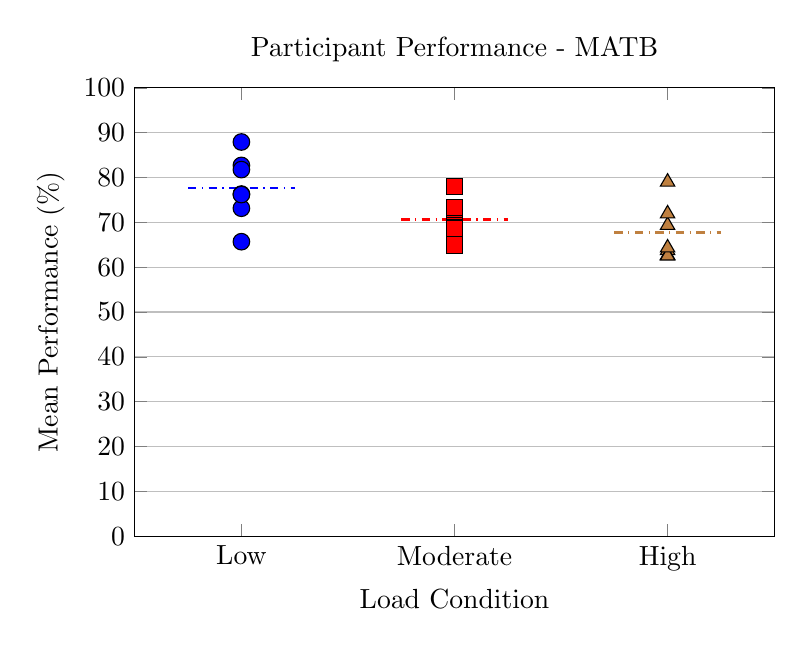
\begin{tikzpicture}
\begin{axis}[
	ymajorgrids,
	width=0.8\textwidth,
	height=0.6\textwidth,
	scatter/classes= {
		a={mark=*, fill=blue, draw=black, mark size=3},
		b={mark=square*, fill=red, draw=black, mark size=3},
		c={mark=triangle*, fill=brown, draw=black, mark size=3},
		d={mark=diamond*, fill=gray, draw=black, mark size=3}
	},
	ymin=0,
	ymax=100,
	xmin=0.5,
	xmax=3.5,
	ytick={0,10,...,100},
	xtick={1,2,3},
	xticklabel style={align=center},
	xticklabels={Low, Moderate, High},
	title=Participant Performance - MATB, 
	ylabel=Mean Performance (\%),
	xlabel=Load Condition]

	% Low
	\addplot+[ scatter,
			only marks,
			scatter src=explicit symbolic]
	coordinates {
			(1, 76.31)	[a]
			(1, 65.69)	[a]
			(1, 82.70)	[a]
			(1, 73.15)	[a]
			(1, 87.93)	[a]
			(1, 76.20)	[a]
			(1, 81.77)	[a]
};

\addplot+[ mark=None, dashdotted, blue, line width = 1pt ] 
	coordinates {
		(0.75, 77.68)
		(1.25, 77.68)
};

	% Moderate
	\addplot+[ scatter,
			only marks,
			scatter src=explicit symbolic]
	coordinates {
			(2, 67.14)	[b]
			(2, 64.98)	[b]
			(2, 69.17)	[b]
			(2, 68.68)	[b]
			(2, 72.87)	[b]
			(2, 73.29)	[b]
			(2, 78.01)	[b]
};
\addplot+[ mark=None, dashdotted, red, line width = 1pt ] 
	coordinates {
		(1.75, 70.59)
		(2.25, 70.59)
};

	% High
	\addplot+[ scatter,
			only marks,
			scatter src=explicit symbolic]
	coordinates {
			(3, 63.74)	[c]
			(3, 62.69)	[c]
			(3, 62.53)	[c]
			(3, 64.33)	[c]
			(3, 69.36)	[c]
			(3, 71.93)	[c]
			(3, 79.02)	[c]
};
\addplot+[ mark=None, dashdotted, brown, line width = 1pt ] 
	coordinates {
		(2.75, 67.66)
		(3.25, 67.66)
};


\end{axis}
\end{tikzpicture}

\end{document}
















